%----------------------------------------------------------------------------------------
%	PACKAGES AND DOCUMENT CONFIGURATIONS
%----------------------------------------------------------------------------------------
\documentclass{article}

\usepackage{graphicx} 	% Required for the inclusion of images
\usepackage{natbib} 	% Required to change bibliography style to APA
\usepackage{amsmath} 	% Required for some math elements 
\usepackage{cases} 
\usepackage{array}
\usepackage{caption}
\usepackage{subcaption}

\usepackage{xcolor}
\usepackage{listings}
\usepackage{color}		 %red, green, blue, yellow, cyan, magenta, black, white
\usepackage{geometry}
\geometry{
a4paper,
total={170mm,257mm},
left=20mm,
top=20mm,
}
\setlength\parindent{0pt} % Removes all indentation from paragraphs

\definecolor{codegreen}{rgb}{0,0.6,0}
\definecolor{codegray}{rgb}{0.5,0.5,0.5}
\definecolor{codepurple}{rgb}{0.58,0,0.82}
\definecolor{backcolour}{rgb}{0.9,0.9,0.9}

\lstdefinestyle{mystyle}{
    %backgroundcolor=\color{backcolour},   
    frame=tb, 				% draw a frame at the top and bottom of the code block
    commentstyle=\color{codegreen},
    keywordstyle=\color{magenta},
    numberstyle=\tiny\color{codegray},
    stringstyle=\color{codepurple},
    basicstyle=\footnotesize,
    breakatwhitespace=false,         
    breaklines=true,                 
    captionpos=b,                    
    keepspaces=true,                 
    numbers=left,                    
    numbersep=5pt,                  
    showspaces=false,                
    showstringspaces=false,
    showtabs=false,                  
    tabsize=4
}
\lstset{style=mystyle}


%----------------------------------------------------------------------------------------
%	DOCUMENT INFORMATION
%----------------------------------------------------------------------------------------
\title{Artificial Intelligence in Control Engineering exercise}
\author{
	Lecturer: Dr.Pham Viet Cuong	\\
}
\date{October 08th, 2018}

\begin{document}
\maketitle 					% Insert the title, author and date

\begin{center}
	\begin{tabular}{l l}
	Group 9: \\
	Nguyen Chinh Thuy 	& 1513372	\\
	Nguyen Tan Phu		& 1512489	\\
	Le Van Hoang Phuong	& 1512579	\\
	Do Tieu Thien		& 1513172			\\
	Nguyen Tan Sy		& 1512872	\\
	Nguyen Van Qui		& 1512702
	\end{tabular}
\end{center}


%----------------------------------------------------------------------------------------
%	SECTION 1
%----------------------------------------------------------------------------------------
\section{Problem}

%----------------------------------------------------------------------------------------
%	SECTION 2
%----------------------------------------------------------------------------------------
\section{Configuration}

%----------------------------------------------------------------------------------------
%	SECTION 3
%----------------------------------------------------------------------------------------
\section{Implementation}
\subsection{Particle Filter}
To solve the Paticle Filter problem, we implement follow below steps: \\
\begin{itemize}
	\item{Prediction} 
	\begin{itemize}
		\begin{subequations} 
		Process model:
		\begin{align}
			x_t = x_{t-1} + V_t\Delta{t}\cos\left({\theta_t + \varphi_{t-1}}\right) \\
			y_t = y_{t-1} + V_t\Delta{t}\cos\left({\theta_t + \varphi_{t-1}}\right) \\
			\varphi_t = \varphi_{t-1} + \dfrac{V_t\Delta{t}\sin{\theta_t}}{WB}
		\end{align}
		\end{subequations}
		\begin{subequations}
		Measurement model:
		\begin{align}
			r_t = \sqrt{{\left(x_t - x_L\right)}^2 + {\left(y_t - y_L\right)}^2}\\
			b_t = \arctan{\dfrac{y_t - y_L}{x_t - x_L}} + \varphi_t
		\end{align}
		\end{subequations}
		\item{Measurement model}
		\item{Implementing a loop with $M$ step which is numbers of particles}
		\item{Using process model and control signals $u_t$ in \textbf{VG} which are affected by thermal noise to calculate coordinate $x^{[m]}_t$ of robot.}
		\item{Combining coordinate of robot from above step and coordinate of landmarks in \textbf{lm} to calculate range $r_t$ and bearing angle $b_t$.}
		\item{Calculating importance factor $w^{[m]}_t$ depend on probability density function fomula with $\mu$ is matrix of expected range and bearing which are from \textbf{Z}.}
		\begin{align}
			f_x(x_1,x_2,...,x_N) = \dfrac{1}{\left(2\pi\right)^{\dfrac{N}{2}}\Vert\Sigma\Vert^{\dfrac{1}{2}}}exp\left(\dfrac{-1}{2}\left(x-\mu\right)^T\Sigma^{-1}\left(x-\mu\right)\right)
		\end{align}
	\end{itemize}
	\item{Selection}
	\begin{itemize}
		\item{Implementing a loop with $M$ step.}
		\item{Choosing a index in range $\left[1,M\right]$ for $x^{[m]}_t$ with probabilities $w^{[m]}_t$.}
	\end{itemize}
\end{itemize}
\subsubsection{Python code}
\lstinputlisting[language=Python]
{../main.py}

%----------------------------------------------------------------------------------------
%	SECTION 4
%----------------------------------------------------------------------------------------
\subsubsection{Result} 
\begin{figure}[h!]
\centering
\begin{subfigure}[b]{0.7\linewidth}
	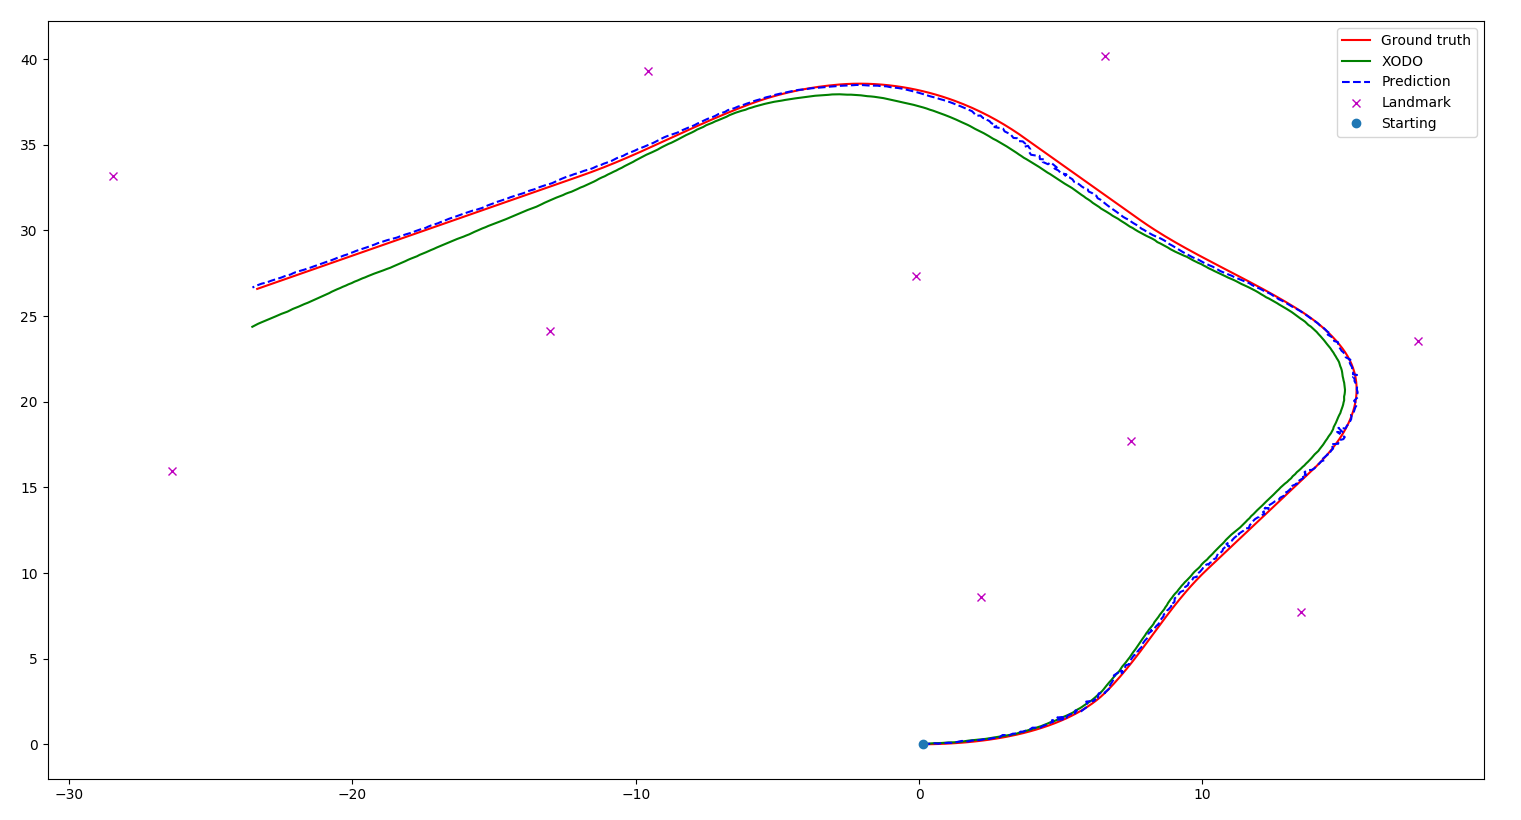
\includegraphics[width=\textwidth]{../max.png}
	\caption{Trajectories with max $w_t$. $RMS = 11.289769$}\label{fig:image-1}
\end{subfigure}
\begin{subfigure}[b]{0.7\linewidth}
	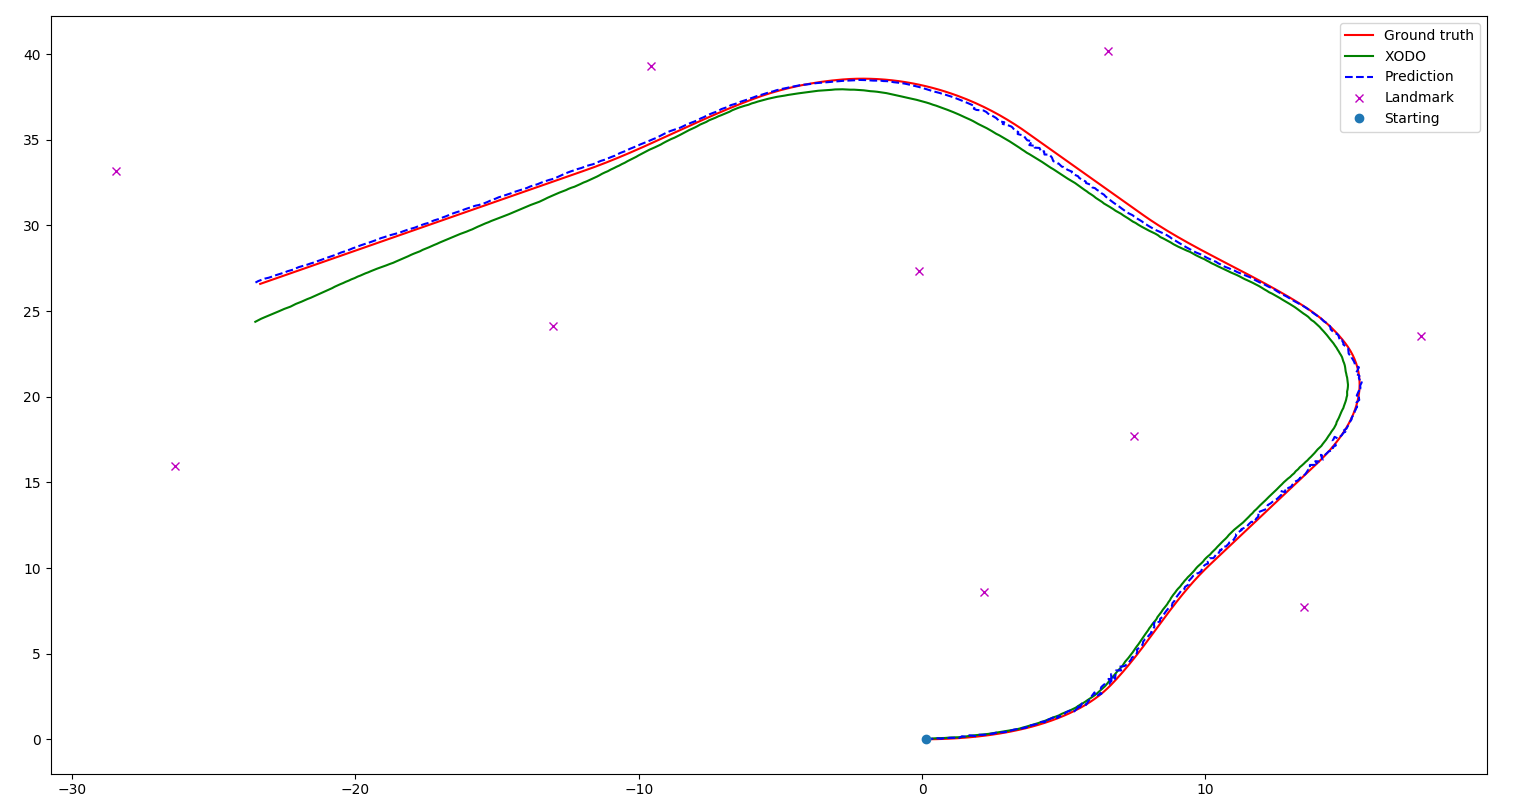
\includegraphics[width=\textwidth]{../median.png}
	\caption{Trajectories with median $w_t$. $RMS = 11.428931$}\label{fig:image-2}
\end{subfigure}
\begin{subfigure}[b]{0.7\linewidth}
	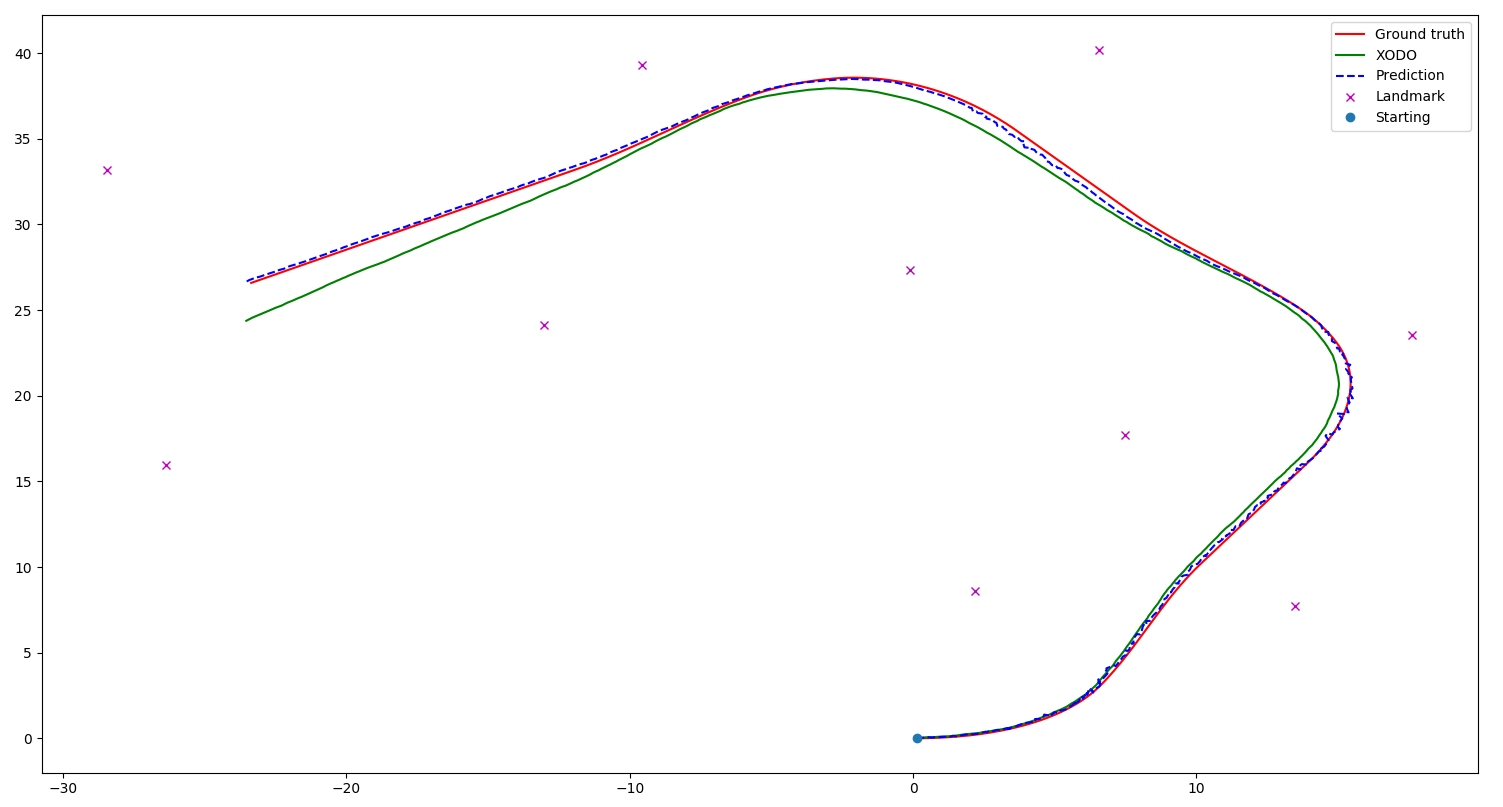
\includegraphics[width=\textwidth]{../min.png}
	\caption{Trajectories with min $w_t$. $RMS = 11.475249$}\label{fig:image-3}
\end{subfigure}
\caption{Trajectories of Ground truth (XTRUE), XODO, Prediction and root mean square (RMS) of Prediction compared to Ground truth.}
\end{figure}
\begin{itemize}
	\item{Comment:}
	\begin{itemize}
		\item{Overall, three trajectories of Prediction fits Ground truth with the same patterns. However, the best fit is belong to trajectoty with choosing max $w_t$, so the root mean square is smallest.} 
		\item{Line of XODO which is calculated from process model is different from Ground truth because of effect on range and bearing angle from thermal noise, while Prediction is calculated and chosen with importance factor $w_t$. That is the reason why line of Prediction is better than XODO.}
	\end{itemize}
\end{itemize}
\end{document} 


